\documentclass[11pt,a4paper]{article}

\usepackage[utf8]{inputenc}
\usepackage[T1]{fontenc}
\usepackage{lmodern}
\usepackage[margin=1in]{geometry}
\usepackage{amsmath,amssymb,amsfonts}
\usepackage{booktabs}
\usepackage{graphicx}
\usepackage{xcolor}
\usepackage{hyperref}
\usepackage{microtype}
\usepackage{caption}
\usepackage{subcaption}
\usepackage{float}
\usepackage{titlesec}
\usepackage{enumitem}

% Hyperref configuration
\hypersetup{
    colorlinks=true,
    linkcolor=blue!70!black,
    citecolor=blue!70!black,
    urlcolor=blue!70!black
}

% Section title formatting
\titleformat{\section}{\large\bfseries}{\thesection}{1em}{}
\titleformat{\subsection}{\normalsize\bfseries}{\thesubsection}{1em}{}
\titleformat{\subsubsection}{\small\bfseries}{\thesubsubsection}{1em}{}

\begin{document}

% ---------------------------------------------------------
% Header & Title
% ---------------------------------------------------------
\begin{center}
    {\scshape\large Deep Learning CSC403-8 --- CIA 1: Component I A}\\[0.5em]
    {\LARGE\bfseries Design, Implementation, and Comparative Analysis of Artificial Neural Networks for Early Diabetes Risk Prediction}\\[0.8em]
    {\large\bfseries Pragya}\\[0.3em]
    {\normalsize Department of Computer Science, School of Computing}\\[0.3em]
    {\normalsize\texttt{Academic Year 2026--2027}}
\end{center}
\vspace{0.8em}
\hrule
\vspace{1em}

% ---------------------------------------------------------
% Abstract
% ---------------------------------------------------------
\begin{abstract}
Early and automated detection of type 2 diabetes mellitus is crucial for preventing irreversible microvascular and macrovascular complications. In this study, we present a rigorous, end-to-end deep learning framework for early diabetes risk classification on the benchmark Pima Indians Diabetes Dataset ($N=768$). We institute a strict, leakage-free data engineering pipeline: physiologically implausible zero readings across five clinical indicators are treated as missing values, partitioned via a stratified 70/15/15 train/validation/test protocol ($N_{\text{train}}=537$, $N_{\text{val}}=115$, $N_{\text{test}}=116$), and imputed using training-split column medians alongside training-fitted standard score normalisation. We design and implement configurable multilayer perceptron (MLP) architectures in PyTorch, exploring activation dynamics (ReLU, LeakyReLU, and Tanh) and structural capacity variants (Shallow, Standard, and Deep Regularised). Controlled benchmarks across five experimental configurations demonstrate that Model~A (ReLU with hidden dimensions $[32, 16]$, dropout rate $p=0.2$, and $L_2$ weight decay $\lambda=10^{-4}$) achieves superior convergence and balanced performance, reaching an optimal validation loss of $0.5028$ at epoch 9 and held-out test metrics of 75.00\% Accuracy, 70.00\% Precision, 51.22\% Recall, 0.5915 F1-Score, and 0.8459 ROC-AUC. Deep regularised architecture (Model~E, $[64, 32, 16]$) achieved the lowest validation loss ($0.4992$) and highest discrimination capability (0.8637 ROC-AUC). We analyse the critical precision-recall trade-off under class imbalance ($34.90\%$ positive prevalence) and discuss clinical deployment requirements, including threshold calibration, cost-sensitive loss functions, and interactive diagnostic software.
\end{abstract}

\vspace{0.5em}
\noindent\textbf{Keywords:} Artificial Neural Networks, Deep Learning, Multilayer Perceptron, Pima Indians Diabetes, Binary Classification, Data Leakage Prevention, Medical Informatics.

\vspace{1em}
\hrule
\vspace{1.2em}

% ---------------------------------------------------------
% Section 1: Problem Formulation and Dataset Description
% ---------------------------------------------------------
\section{Problem Formulation and Dataset Description}
\label{sec:problem_formulation}

\subsection{Clinical Motivation and Mathematical Formulation}
Type 2 diabetes is a chronic metabolic disorder characterised by chronic hyperglycaemia resulting from insulin resistance or relative insulin deficiency. According to epidemiological surveillance, early lifestyle or pharmacological intervention significantly attenuates disease progression and reduces the incidence of diabetic retinopathy, nephropathy, and cardiovascular mortality. 

We formulate early diabetes risk prediction as a supervised binary classification task. Let $\mathcal{D} = \{(\mathbf{x}_i, y_i)\}_{i=1}^N$ denote a dataset of $N=768$ patient records, where each patient observation is an 8-dimensional feature vector $\mathbf{x}_i \in \mathbb{R}^8$ representing non-invasive and routine clinical biomarkers, and $y_i \in \{0, 1\}$ denotes the diagnostic outcome:
\begin{equation}
    y_i = \begin{cases} 
        1, & \text{if patient tested positive for diabetes within 5 years of examination,} \\ 
        0, & \text{otherwise.} 
    \end{cases}
\end{equation}
The statistical objective is to parameterise an artificial neural network hypothesis $f_{\boldsymbol{\theta}}: \mathbb{R}^8 \to [0, 1]$, parameterised by weight tensors and bias vectors $\boldsymbol{\theta} = \{\mathbf{W}^{(l)}, \mathbf{b}^{(l)}\}_{l=1}^L$, that outputs the posterior probability $\hat{y}_i = P(y_i = 1 \mid \mathbf{x}_i; \boldsymbol{\theta})$ while minimising the empirical risk regularised by parameter complexity.

\subsection{Dataset Characteristics and Biologically Invalid Zeros}
The dataset analysed is the benchmark Pima Indians Diabetes Dataset from the National Institute of Diabetes and Digestive and Kidney Diseases (NIDDK) \cite{smith1988using}. It comprises records of 768 female patients of Pima Indian heritage aged 21 years and older. The cohort exhibits an inherent class imbalance: 500 patients (65.10\%) are non-diabetic ($y=0$), whereas 268 patients (34.90\%) are diagnosed with diabetes ($y=1$), establishing an imbalance ratio of $1.87:1$.

A critical vulnerability in raw medical datasets is the encoding of missing measurements as numerical zeros. While a value of zero is biologically valid for \texttt{Pregnancies} (representing nulliparous women, observed in 111 patients), numerical zeros in physiological features such as plasma glucose concentration, diastolic blood pressure, triceps skinfold thickness, 2-hour serum insulin, and body mass index (BMI) are incompatible with human survival. Treating these as true numerical zero values introduces severe distributional distortion and biases artificial neuron activations.

\begin{table}[H]
    \centering
    \small
    \caption{Summary of Clinical Features, Missing (Zero) Value Counts, and Training Set Median Imputation Statistics ($N=768$, Training Split $N_{\text{train}}=537$).}
    \label{tab:features_summary}
    \begin{tabular}{@{}llccrc@{}}
        \toprule
        \textbf{Feature Name} & \textbf{Clinical Description} & \textbf{Unit} & \textbf{Invalid Zeros} & \textbf{Missing (\%)} & \textbf{Train Median} \\
        \midrule
        \texttt{Pregnancies} & Number of times pregnant & Count & 0 (111 valid) & 0.00\% & 3.00 \\
        \texttt{Glucose} & 2-hr oral glucose tolerance test & mg/dL & 5 & 0.65\% & 117.00 \\
        \texttt{BloodPressure} & Diastolic blood pressure & mm Hg & 35 & 4.56\% & 72.00 \\
        \texttt{SkinThickness} & Triceps skinfold thickness & mm & 227 & 29.56\% & 29.00 \\
        \texttt{Insulin} & 2-hour serum insulin & $\mu$U/mL & 374 & 48.70\% & 126.00 \\
        \texttt{BMI} & Body mass index & $\text{kg/m}^2$ & 11 & 1.43\% & 32.40 \\
        \texttt{DiabetesPedigree} & Genetic diabetes family pedigree & Score & 0 & 0.00\% & 0.385 \\
        \texttt{Age} & Age of patient & Years & 0 & 0.00\% & 30.00 \\
        \midrule
        \texttt{Outcome} & Clinical diagnostic class & Binary & 500 (Class 0) & 268 (Class 1) & 34.90\% Pos. \\
        \bottomrule
    \end{tabular}
\end{table}

\subsection{Leakage-Free Preprocessing Pipeline}
To guarantee rigorous generalization and prevent data leakage, our preprocessing pipeline enforces strict separation between training, validation, and test splits:
\begin{enumerate}[leftmargin=*]
    \item \textbf{Invalid Zero Replacement:} Numerical zeros in $[\texttt{Glucose}, \texttt{BloodPressure}, \texttt{SkinThickness}, \texttt{Insulin}, \texttt{BMI}]$ are explicitly converted to IEEE \texttt{NaN} prior to any statistical computations.
    \item \textbf{Stratified Splitting:} The dataset is partitioned using a stratified 70/15/15 ratio (with deterministic seed 42) into:
    \begin{itemize}
        \item Training set: $N_{\text{train}} = 537$ samples (350 non-diabetic, 187 diabetic; 34.82\% positive prevalence);
        \item Validation set: $N_{\text{val}} = 115$ samples (75 non-diabetic, 40 diabetic; 34.78\% positive prevalence);
        \item Held-out test set: $N_{\text{test}} = 116$ samples (75 non-diabetic, 41 diabetic; 35.34\% positive prevalence).
    \end{itemize}
    \item \textbf{Median Imputation strictly on Training Split:} Column medians $\tilde{\mathbf{x}}_{\text{train}, j}$ are computed exclusively over the training set $\mathcal{D}_{\text{train}}$:
    \begin{equation}
        \tilde{x}_{\text{train}, j} = \text{median}\left(\{x_{i, j} \mid (\mathbf{x}_i, y_i) \in \mathcal{D}_{\text{train}}, x_{i, j} \neq \texttt{NaN}\}\right).
    \end{equation}
    The resulting scalar medians (Table~\ref{tab:features_summary}) are subsequently broadcast to impute missing entries across $\mathcal{D}_{\text{train}}$, $\mathcal{D}_{\text{val}}$, and $\mathcal{D}_{\text{test}}$.
    \item \textbf{Standard Score Scaling:} To prevent gradient dominance by features with large numerical magnitudes (e.g., \texttt{Insulin} $\sim 10^2$ vs.\ \texttt{DiabetesPedigreeFunction} $\sim 10^{-1}$), standardisation parameters are fitted strictly on the imputed training features:
    \begin{equation}
        \mu_j = \frac{1}{N_{\text{train}}} \sum_{i=1}^{N_{\text{train}}} x_{i, j}^{\text{imp}}, \quad \sigma_j = \sqrt{\frac{1}{N_{\text{train}}} \sum_{i=1}^{N_{\text{train}}} (x_{i, j}^{\text{imp}} - \mu_j)^2}.
    \end{equation}
    Features are normalised via $x_{i, j}^{\text{scaled}} = (x_{i, j}^{\text{imp}} - \mu_j) / \sigma_j$. The validation and test features are transformed using $(\boldsymbol{\mu}_{\text{train}}, \boldsymbol{\sigma}_{\text{train}})$, ensuring zero leakage of test distribution statistics into model training.
\end{enumerate}

Figure~\ref{fig:correlation_heatmap} illustrates the Pearson correlation matrix of the preprocessed features. \texttt{Glucose} exhibits the highest linear correlation with \texttt{Outcome} ($r = 0.49$), followed by \texttt{BMI} ($r = 0.31$) and \texttt{Age} ($r = 0.24$). Inter-feature collinearity is notable between \texttt{SkinThickness} and \texttt{BMI} ($r = 0.54$) and between \texttt{Pregnancies} and \texttt{Age} ($r = 0.54$).

\begin{figure}[H]
    \centering
    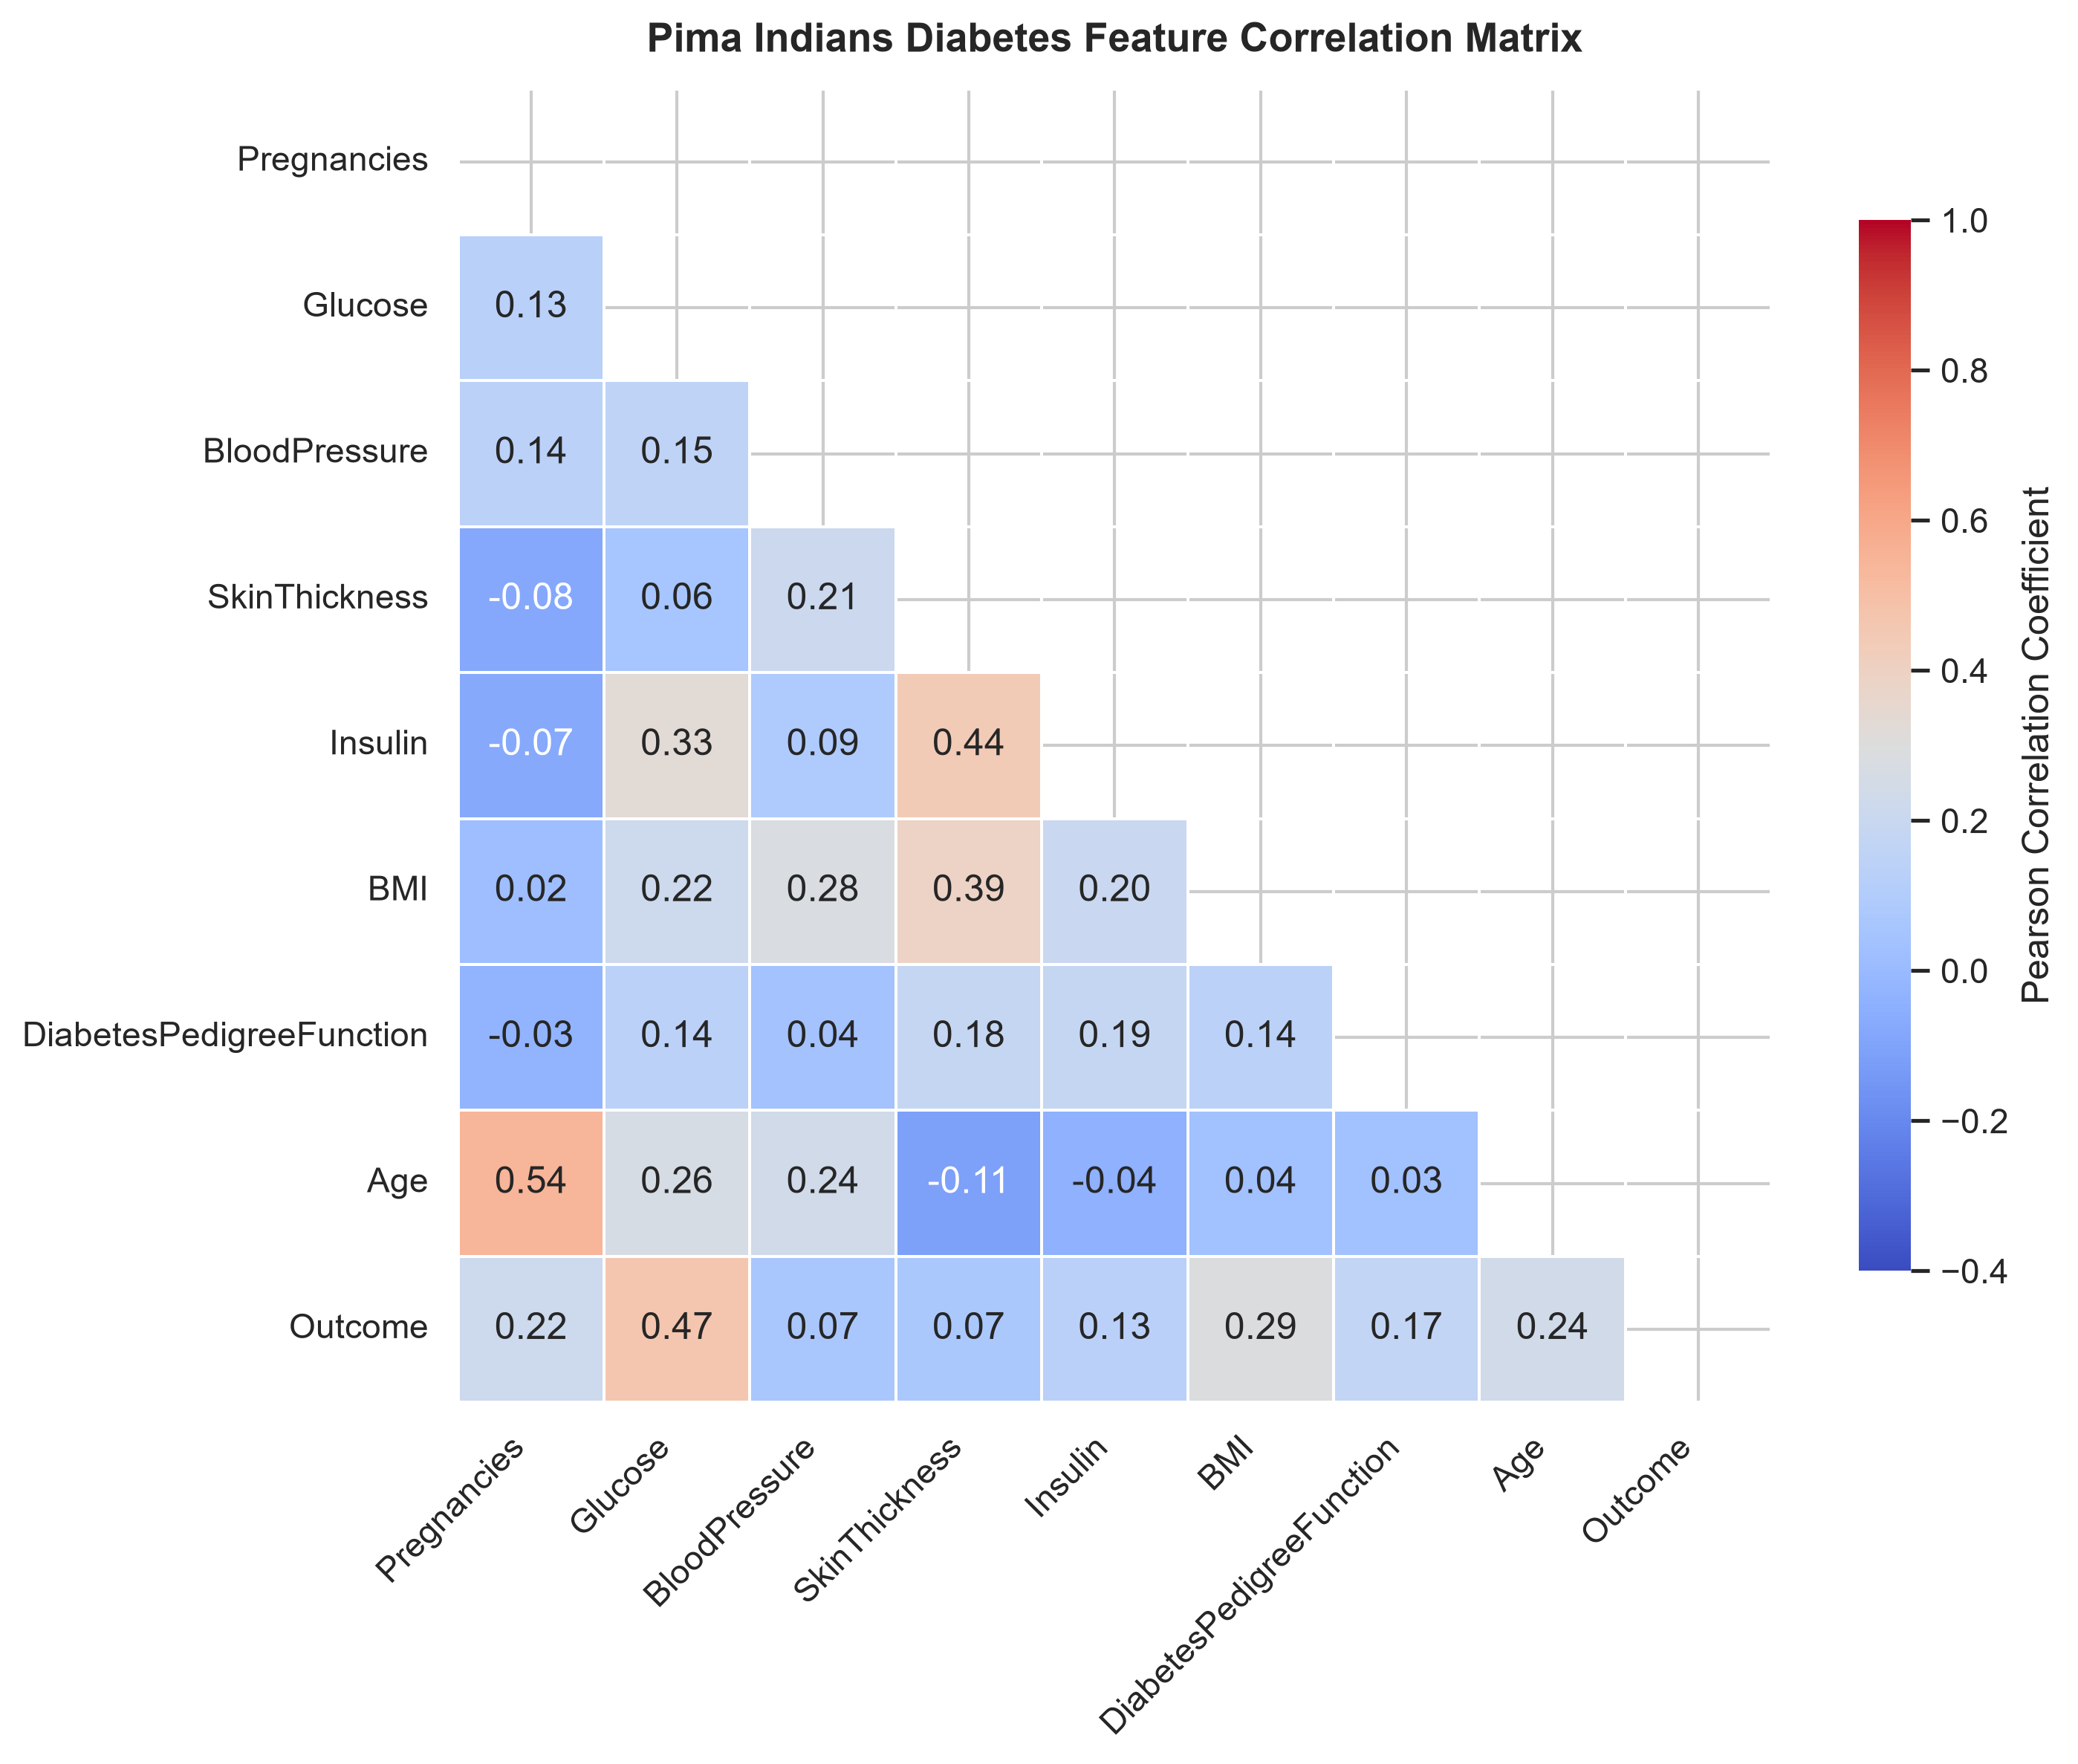
\includegraphics[width=0.72\textwidth]{figures/correlation_heatmap.png}
    \caption{Pearson correlation heatmap across all 8 preprocessed clinical features and the binary target \texttt{Outcome}.}
    \label{fig:correlation_heatmap}
\end{figure}

% ---------------------------------------------------------
% Section 2: Mathematical Modelling of Artificial Neurons
% ---------------------------------------------------------
\section{Mathematical Modelling of Artificial Neurons}
\label{sec:math_modelling}

\subsection{Forward Propagation in a Multilayer Perceptron}
Consider an $L$-layer Multilayer Perceptron (MLP) with input dimension $d_0 = 8$, hidden layer dimensions $d_1, d_2, \dots, d_{L-1}$, and scalar output dimension $d_L = 1$. Let $\mathbf{a}^{(0)} = \mathbf{x} \in \mathbb{R}^8$ denote the input vector. For each layer $l \in \{1, 2, \dots, L\}$, the pre-activation vector $\mathbf{z}^{(l)} \in \mathbb{R}^{d_l}$ is computed via an affine transformation:
\begin{equation}
    \mathbf{z}^{(l)} = \mathbf{W}^{(l)} \mathbf{a}^{(l-1)} + \mathbf{b}^{(l)},
    \label{eq:affine}
\end{equation}
where $\mathbf{W}^{(l)} \in \mathbb{R}^{d_l \times d_{l-1}}$ is the weight matrix and $\mathbf{b}^{(l)} \in \mathbb{R}^{d_l}$ is the bias vector. The post-activation representation $\mathbf{a}^{(l)} \in \mathbb{R}^{d_l}$ is obtained by applying an element-wise non-linear activation function $g^{(l)}(\cdot)$:
\begin{equation}
    \mathbf{a}^{(l)} = g^{(l)}(\mathbf{z}^{(l)}).
    \label{eq:activation}
\end{equation}
For hidden layers $l \in \{1, \dots, L-1\}$, dropout regularization is applied during training:
\begin{equation}
    \tilde{\mathbf{a}}^{(l)} = \frac{\mathbf{r}^{(l)} \odot \mathbf{a}^{(l)}}{1 - p}, \quad r_j^{(l)} \sim \text{Bernoulli}(1 - p),
\end{equation}
where $p \in [0, 1)$ is the dropout probability and $1/(1-p)$ preserves expected activation magnitude.

\subsection{Activation Functions and Analytical Derivatives}
Non-linear activation functions enable the network to construct complex non-linear decision boundaries. We evaluate three distinct activations:

\subsubsection{Rectified Linear Unit (ReLU)}
ReLU maps negative inputs to zero while preserving positive inputs linearly:
\begin{equation}
    g_{\text{ReLU}}(z) = \max(0, z), \quad 
    g'_{\text{ReLU}}(z) = \begin{cases} 
        1, & z > 0, \\ 
        0, & z < 0. 
    \end{cases}
\end{equation}
At $z=0$, the subgradient is conventionally set to 0. ReLU provides scale-invariant gradients for $z>0$, avoiding vanishing gradients, though neurons whose pre-activations remain negative across all training examples can suffer from the ``dying ReLU'' failure mode.

\subsubsection{Leaky Rectified Linear Unit (LeakyReLU)}
To prevent irreversible gradient extinction in negative domains, LeakyReLU introduces a fixed non-zero slope $\alpha = 0.01$:
\begin{equation}
    g_{\text{LeakyReLU}}(z) = \max(\alpha z, z), \quad 
    g'_{\text{LeakyReLU}}(z) = \begin{cases} 
        1, & z > 0, \\ 
        \alpha, & z \leq 0. 
    \end{cases}
\end{equation}
This ensures a continuous, non-zero gradient $\alpha = 0.01$ throughout the backpropagation phase for negative activations.

\subsubsection{Hyperbolic Tangent (Tanh)}
The Tanh activation produces zero-centred, bounded outputs in the interval $(-1, 1)$:
\begin{equation}
    g_{\text{Tanh}}(z) = \tanh(z) = \frac{e^z - e^{-z}}{e^z + e^{-z}}, \quad 
    g'_{\text{Tanh}}(z) = 1 - \tanh^2(z) = 1 - [g_{\text{Tanh}}(z)]^2.
\end{equation}
Because the derivative approaches zero as $|z| \to \infty$, Tanh saturates for large inputs, leading to slower convergence compared to non-saturating piecewise linear activations.

\subsection{Output Sigmoid and Binary Cross-Entropy Loss with $L_2$ Regularization}
The final layer produces a single scalar logit $z^{(L)} \in \mathbb{R}$. The posterior probability of diabetes is obtained via the standard logistic sigmoid function $\sigma: \mathbb{R} \to (0, 1)$:
\begin{equation}
    \hat{y} = \sigma(z^{(L)}) = \frac{1}{1 + e^{-z^{(L)}}}, \quad 
    \sigma'(z) = \sigma(z)(1 - \sigma(z)).
\end{equation}
Given target $y \in \{0, 1\}$ and predicted probability $\hat{y}$, the Binary Cross-Entropy (BCE) loss regularised by $L_2$ weight decay (Frobenius norm) is given by:
\begin{equation}
    \mathcal{L}(\boldsymbol{\theta}) = -\frac{1}{N} \sum_{i=1}^N \left[ y_i \ln \hat{y}_i + (1 - y_i) \ln(1 - \hat{y}_i) \right] + \frac{\lambda}{2} \sum_{l=1}^L \|\mathbf{W}^{(l)}\|_F^2,
    \label{eq:bce_loss}
\end{equation}
where $\lambda \geq 0$ is the weight decay penalty parameter and $\|\mathbf{W}^{(l)}\|_F^2 = \sum_{j,k} (W_{j,k}^{(l)})^2$.

To avoid numerical overflow and precision underflow when computing $\ln \sigma(z)$ for large negative logits, PyTorch implements \texttt{BCEWithLogitsLoss} by combining the sigmoid and logarithm via the log-sum-exp trick:
\begin{equation}
    \ell(z_i, y_i) = \max(z_i, 0) - z_i y_i + \ln\left(1 + e^{-|z_i|}\right).
\end{equation}

\subsection{Backpropagation and Gradient Updates}
The backpropagation algorithm evaluates exact parameter gradients via the chain rule. Defining the local error vector at layer $l$ as $\boldsymbol{\delta}^{(l)} \triangleq \frac{\partial \mathcal{L}}{\partial \mathbf{z}^{(l)}}$:
\begin{itemize}[leftmargin=*]
    \item \textbf{Output Layer Error:} For the scalar logit $z^{(L)}$ with sigmoid output and BCE loss:
    \begin{equation}
        \delta^{(L)} = \frac{\partial \mathcal{L}}{\partial \hat{y}} \cdot \frac{\partial \hat{y}}{\partial z^{(L)}} = \left( -\frac{y}{\hat{y}} + \frac{1 - y}{1 - \hat{y}} \right) \cdot \hat{y}(1 - \hat{y}) = \hat{y} - y = \sigma(z^{(L)}) - y.
        \label{eq:output_error}
    \end{equation}
    Remarkably, the non-linear derivative terms cancel out, preventing gradient saturation at the output when using BCE.
    \item \textbf{Hidden Layer Error Propagation:} For $l = L-1, L-2, \dots, 1$:
    \begin{equation}
        \boldsymbol{\delta}^{(l)} = \left( (\mathbf{W}^{(l+1)})^T \boldsymbol{\delta}^{(l+1)} \right) \odot g'(\mathbf{z}^{(l)}),
        \label{eq:hidden_error}
    \end{equation}
    where $\odot$ denotes the Hadamard (element-wise) product.
    \item \textbf{Parameter Gradients:}
    \begin{equation}
        \frac{\partial \mathcal{L}}{\partial \mathbf{W}^{(l)}} = \boldsymbol{\delta}^{(l)} (\mathbf{a}^{(l-1)})^T + \lambda \mathbf{W}^{(l)}, \quad 
        \frac{\partial \mathcal{L}}{\partial \mathbf{b}^{(l)}} = \boldsymbol{\delta}^{(l)}.
    \end{equation}
\end{itemize}

Network parameters are updated using the Adam (Adaptive Moment Estimation) optimizer \cite{kingma2014adam}, which computes exponentially decaying averages of past gradients ($m_t$) and squared gradients ($v_t$) with bias corrections:
\begin{equation}
    \mathbf{m}_t = \beta_1 \mathbf{m}_{t-1} + (1 - \beta_1) \mathbf{g}_t, \quad 
    \mathbf{v}_t = \beta_2 \mathbf{v}_{t-1} + (1 - \beta_2) \mathbf{g}_t^2,
\end{equation}
\begin{equation}
    \hat{\mathbf{m}}_t = \frac{\mathbf{m}_t}{1 - \beta_1^t}, \quad 
    \hat{\mathbf{v}}_t = \frac{\mathbf{v}_t}{1 - \beta_2^t}, \quad 
    \boldsymbol{\theta}_{t+1} = \boldsymbol{\theta}_t - \frac{\eta}{\sqrt{\hat{\mathbf{v}}_t} + \epsilon} \hat{\mathbf{m}}_t,
\end{equation}
with default hyperparameters $\eta = 0.001$, $\beta_1 = 0.9$, $\beta_2 = 0.999$, and $\epsilon = 10^{-8}$.

% ---------------------------------------------------------
% Section 3: ANN Architecture Design and Implementation
% ---------------------------------------------------------
\section{ANN Architecture Design and Implementation}
\label{sec:architecture_design}

\subsection{Modular Codebase Architecture}
The implementation is organized into a clean, modular Python repository adhering to production software engineering standards:
\begin{itemize}[leftmargin=*]
    \item \texttt{src/preprocess.py}: Implements raw CSV ingestion, zero imputation with training medians, stratified splitting ($70/15/15$), StandardScaler fitting, and serialization of joblib scaler, JSON metadata, and NumPy arrays.
    \item \texttt{src/model.py}: Contains the configurable PyTorch module \texttt{DiabetesMLP(nn.Module)}. It features dynamic layer instantiation, mathematical docstrings mapping every operator to analytical equations, and reflection helper methods (\texttt{get\_layer\_shapes()}, \texttt{get\_trainable\_parameters()}).
    \item \texttt{src/train.py}: Implements deterministic seed setting (\texttt{torch}, \texttt{numpy}, \texttt{random} set to 42), the \texttt{TabularDataset} data loader, mini-batch training loop (batch size 32, max 150 epochs), Adam optimization, validation early stopping with patience $K=15$, and metrics evaluation.
    \item \texttt{src/experiments.py}: Automates controlled experimental protocols across multiple activation functions and structural depths on identical preprocessed splits.
    \item \texttt{app.py}: A Streamlit web application providing dataset metrics, interactive LaTeX equations, benchmark visualization, and live patient risk inference.
\end{itemize}

\subsection{Exact Parameter Count Calculation}
For an MLP with input dimension $d_0$ and $L$ weight layers of dimensions $[d_1, d_2, \dots, d_L]$, the total number of trainable parameters $P$ is given by:
\begin{equation}
    P = \sum_{l=1}^L \left( d_{l-1} \cdot d_l + d_l \right) = \sum_{l=1}^L d_l(d_{l-1} + 1).
\end{equation}

Table~\ref{tab:architecture_comparison} summarizes the three architectural topologies examined in our experiments.

\begin{table}[H]
    \centering
    \small
    \caption{Architectural Specification and Analytical Parameter Count Decomposition.}
    \label{tab:architecture_comparison}
    \begin{tabular}{@{}llccr@{}}
        \toprule
        \textbf{Architecture} & \textbf{Layer Shapes} & \textbf{Weight Shapes} & \textbf{Bias Shapes} & \textbf{Total Params} \\
        \midrule
        \textbf{Shallow (Model D)} & $8 \to 16 \to 1$ & $[16, 8], [1, 16]$ & $[16], [1]$ & $(128+16) + (16+1) = \mathbf{161}$ \\
        \textbf{Standard (Models A, B, C)} & $8 \to 32 \to 16 \to 1$ & $[32, 8], [16, 32], [1, 16]$ & $[32], [16], [1]$ & $(256+32) + (512+16) + (16+1) = \mathbf{833}$ \\
        \textbf{Deep Regularised (Model E)} & $8 \to 64 \to 32 \to 16 \to 1$ & $[64, 8], [32, 64], [16, 32], [1, 16]$ & $[64], [32], [16], [1]$ & $(512+64) + (2048+32) + (512+16) + (16+1) = \mathbf{3{,}201}$ \\
        \bottomrule
    \end{tabular}
\end{table}

% ---------------------------------------------------------
% Section 4: Experimental Analysis and Performance Evaluation
% ---------------------------------------------------------
\section{Experimental Analysis and Performance Evaluation}
\label{sec:experimental_analysis}

\subsection{Evaluation Metrics Formulation}
Given a decision threshold $\tau = 0.50$, predicted probabilities $\hat{y}_i$ are thresholded into binary predictions $\hat{c}_i = \mathbb{I}(\hat{y}_i \geq \tau)$. Performance is evaluated on the independent held-out test split ($N_{\text{test}}=116$) using standard clinical diagnostic metrics:
\begin{itemize}[leftmargin=*]
    \item \textbf{Accuracy:} Overall fraction of correct classifications:
    \begin{equation}
        \text{Accuracy} = \frac{\text{TP} + \text{TN}}{\text{TP} + \text{TN} + \text{FP} + \text{FN}}.
    \end{equation}
    \item \textbf{Precision (Positive Predictive Value, PPV):} Probability that a positive test indicates true diabetes:
    \begin{equation}
        \text{Precision} = \frac{\text{TP}}{\text{TP} + \text{FP}}.
    \end{equation}
    \item \textbf{Recall (Sensitivity):} Probability that a true diabetic patient is correctly flagged by the model:
    \begin{equation}
        \text{Recall} = \frac{\text{TP}}{\text{TP} + \text{FN}}.
    \end{equation}
    \item \textbf{F1-Score:} Harmonic mean of precision and recall:
    \begin{equation}
        \text{F1-Score} = 2 \cdot \frac{\text{Precision} \cdot \text{Recall}}{\text{Precision} + \text{Recall}} = \frac{2\text{TP}}{2\text{TP} + \text{FP} + \text{FN}}.
    \end{equation}
    \item \textbf{ROC-AUC:} Area under the Receiver Operating Characteristic curve, computing the probability that the classifier ranks a randomly chosen diabetic patient higher than a non-diabetic patient:
    \begin{equation}
        \text{ROC-AUC} = \int_{0}^1 \text{TPR}(\text{FPR}^{-1}(u)) \, du.
    \end{equation}
\end{itemize}

\subsection{Controlled Experimental Results}
All models were trained using deterministic seeds (42) with batch size 32, Adam optimizer ($\eta=0.001$), maximum 150 epochs, and early stopping on validation loss with patience $K=15$.
\begin{itemize}[leftmargin=*]
    \item \textbf{Experiment Set 1 (Activation Functions):} Hidden layers $[32, 16]$, dropout $p=0.2$, weight decay $\lambda=10^{-4}$. Compares ReLU (Model A), LeakyReLU (Model B), and Tanh (Model C).
    \item \textbf{Experiment Set 2 (Architecture and Regularization):} Evaluates capacity scaling using the winning activation from Set 1 (ReLU). Compares Shallow (Model D: $[16]$, $p=0$, $\lambda=0$) against Deep Regularised (Model E: $[64, 32, 16]$, $p=0.3$, $\lambda=10^{-4}$).
\end{itemize}

Table~\ref{tab:comparison_table} presents the exact experimental metrics extracted from our benchmark runs on the held-out test split.

\begin{table}[H]
    \centering
    \small
    \caption{Complete Benchmark Results Across 5 Controlled ANN Configurations on the Held-Out Test Set ($N_{\text{test}}=116$, Seed=42). Best values within each set are highlighted in bold.}
    \label{tab:comparison_table}
    \resizebox{\textwidth}{!}{%
    \begin{tabular}{@{}llcrrrrrrrrr@{}}
        \toprule
        \textbf{Model ID} & \textbf{Architecture} & \textbf{Act.} & \textbf{Params} & \textbf{Best Ep.} & \textbf{Val Loss} & \textbf{Accuracy} & \textbf{Precision} & \textbf{Recall} & \textbf{F1} & \textbf{ROC-AUC} & \textbf{Time (s)} \\
        \midrule
        \multicolumn{12}{@{}l}{\textit{\textbf{Set 1: Activation Function Comparison (Layers: [32, 16], Dropout: 0.2, WD: 1e-4)}}} \\
        \textbf{Model A} & $[32, 16]$ & \textbf{ReLU} & 833 & \textbf{9} & \textbf{0.5028} & \textbf{0.7500} & \textbf{0.7000} & \textbf{0.5122} & \textbf{0.5915} & 0.8459 & 4.18 \\
        \textbf{Model B} & $[32, 16]$ & LeakyReLU & 833 & 9 & 0.5033 & 0.7500 & 0.7000 & 0.5122 & 0.5915 & 0.8455 & 0.87 \\
        \textbf{Model C} & $[32, 16]$ & Tanh & 833 & 48 & 0.5094 & 0.7500 & 0.7000 & 0.5122 & 0.5915 & \textbf{0.8641} & 2.27 \\
        \midrule
        \multicolumn{12}{@{}l}{\textit{\textbf{Set 2: Architecture \& Regularization Comparison (Activation: ReLU)}}} \\
        \textbf{Model D} & $[16]$ & ReLU & 161 & 24 & 0.5090 & 0.7414 & 0.6897 & 0.4878 & 0.5714 & 0.8602 & 1.26 \\
        \textbf{Model E} & $[64, 32, 16]$ & \textbf{ReLU} & 3{,}201 & \textbf{14} & \textbf{0.4992} & \textbf{0.7500} & \textbf{0.7000} & \textbf{0.5122} & \textbf{0.5915} & \textbf{0.8637} & 1.20 \\
        \bottomrule
    \end{tabular}%
    }
\end{table}

\begin{figure}[H]
    \centering
    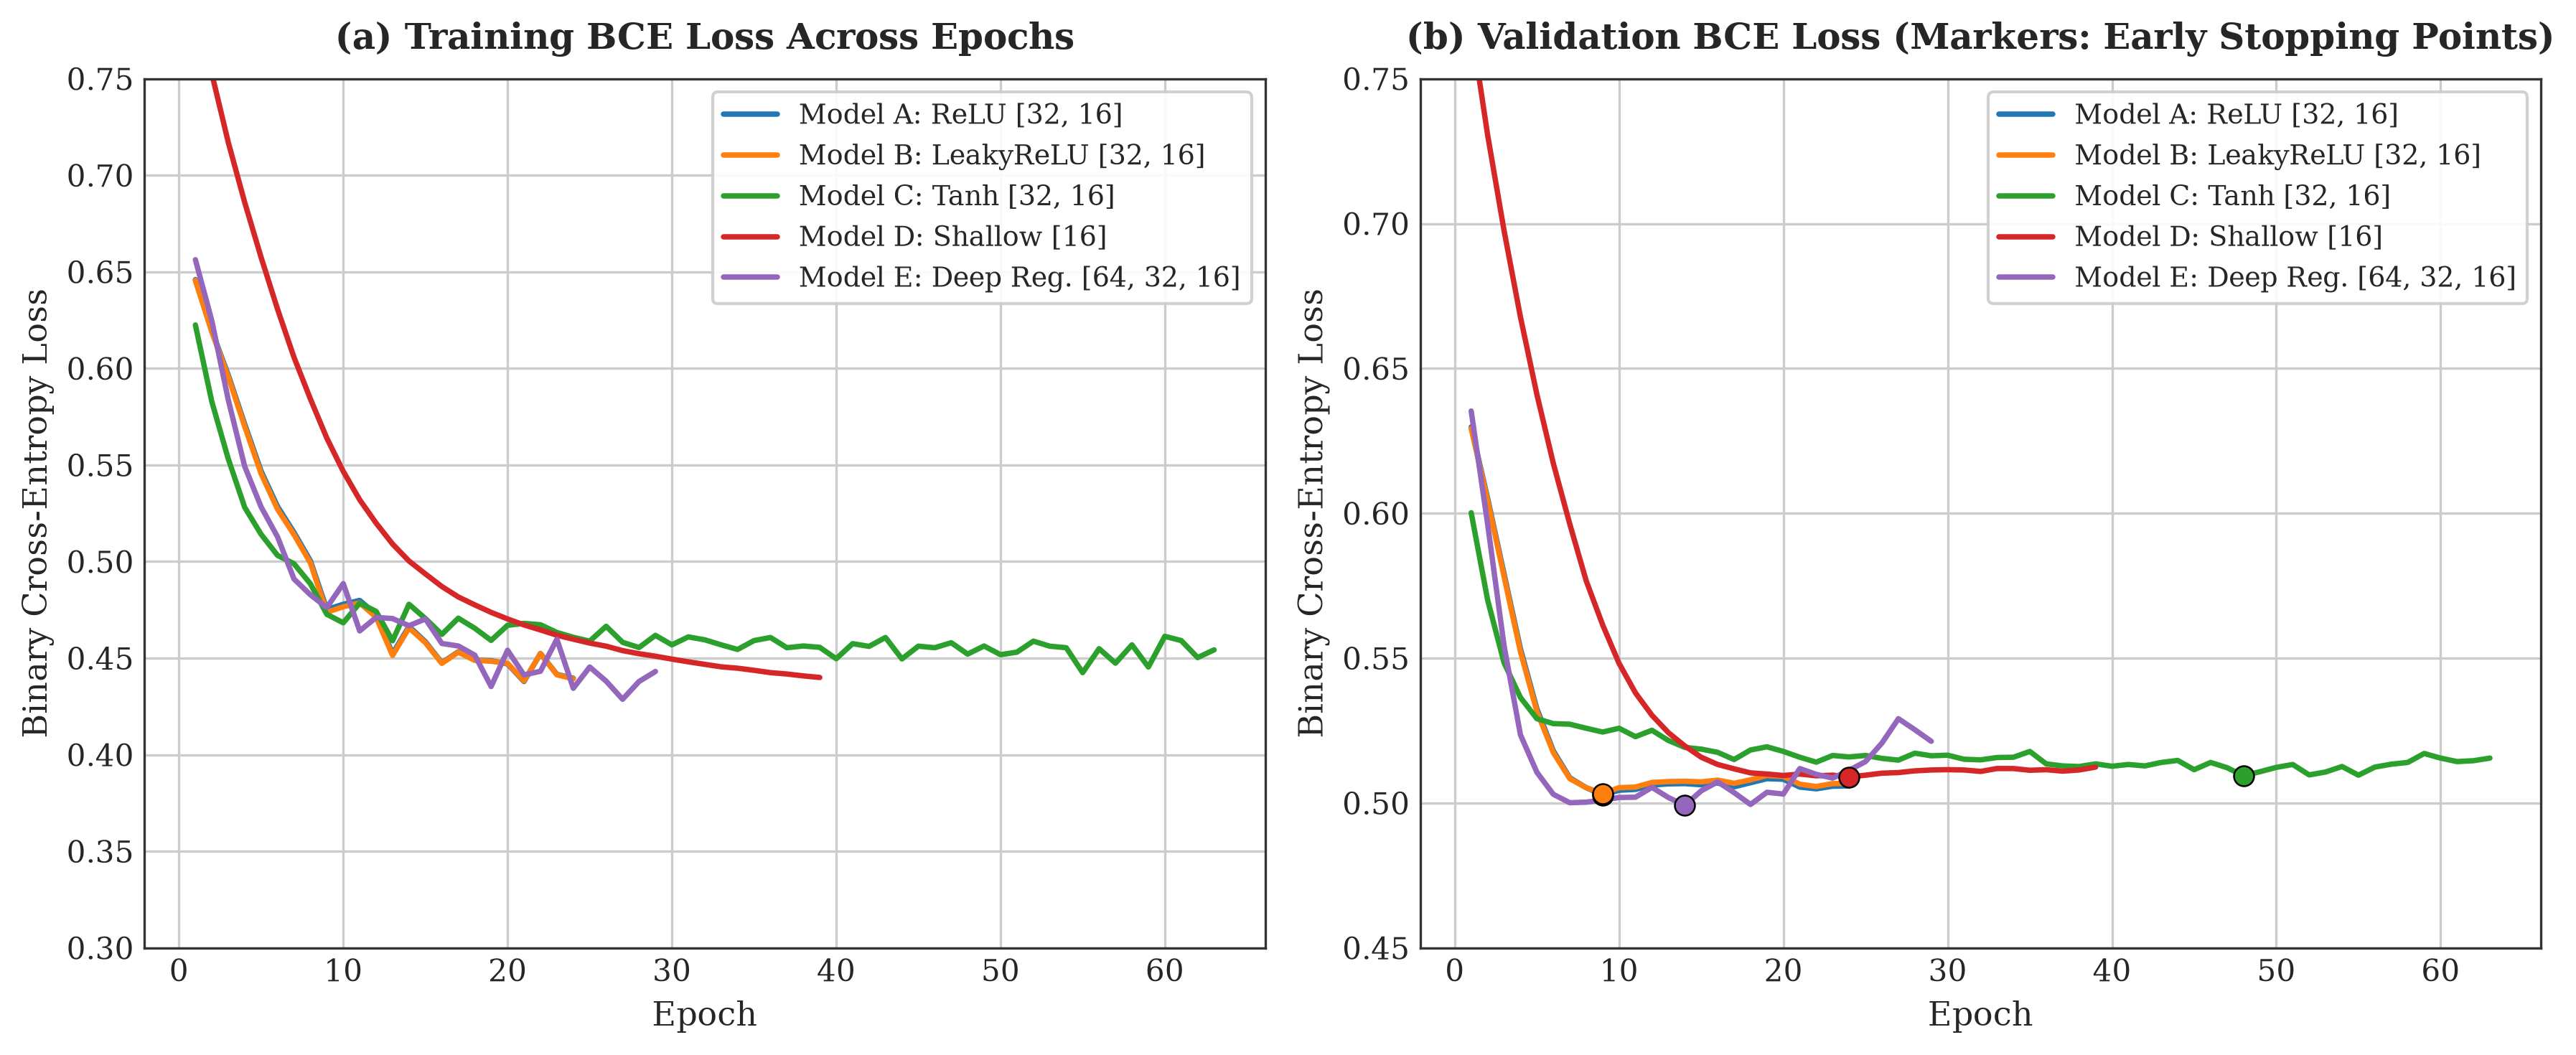
\includegraphics[width=\textwidth]{figures/loss_curves.png}
    \caption{BCE loss trajectories across training and validation splits for all 5 ANN architectures. Markers indicate the best validation epoch where the checkpoint was captured prior to early stopping.}
    \label{fig:loss_curves}
\end{figure}

\begin{figure}[H]
    \centering
    \begin{minipage}{0.48\textwidth}
        \centering
        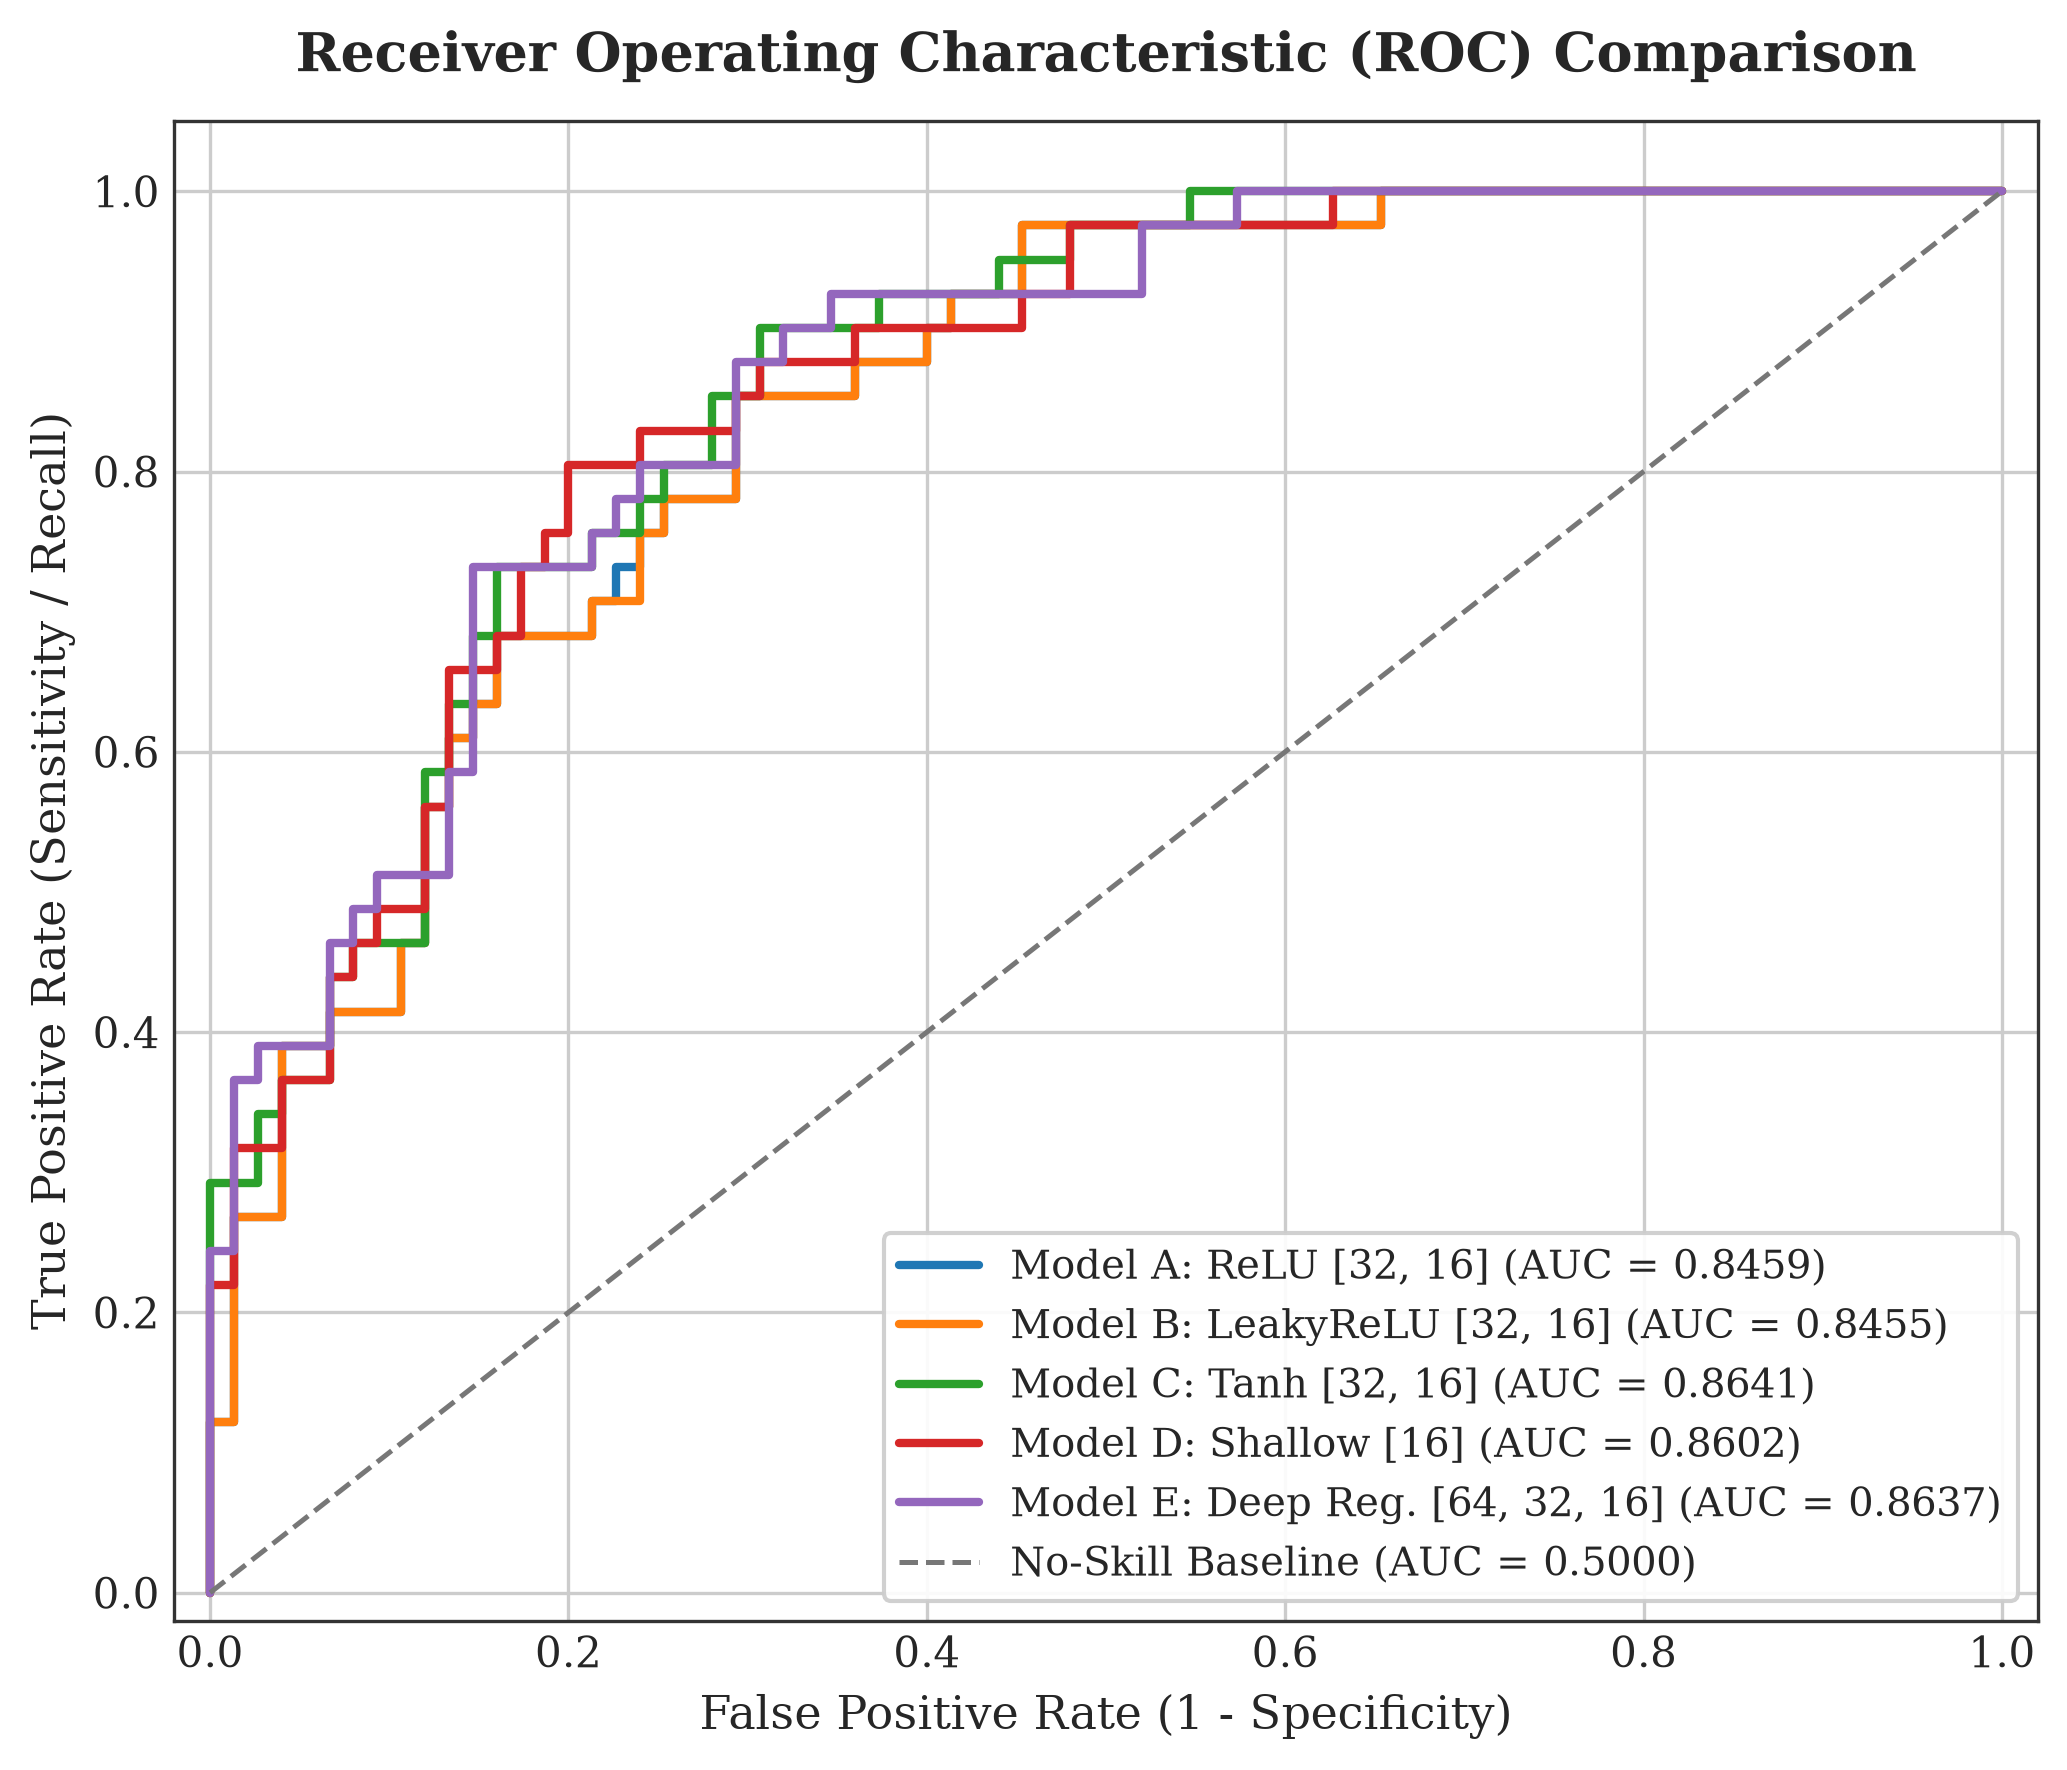
\includegraphics[width=\linewidth]{figures/roc_curves.png}
        \caption{Combined ROC curves for Models A--E on the held-out test split ($N=116$), showing exact ROC-AUC scores.}
        \label{fig:roc_curves}
    \end{minipage}\hfill
    \begin{minipage}{0.48\textwidth}
        \centering
        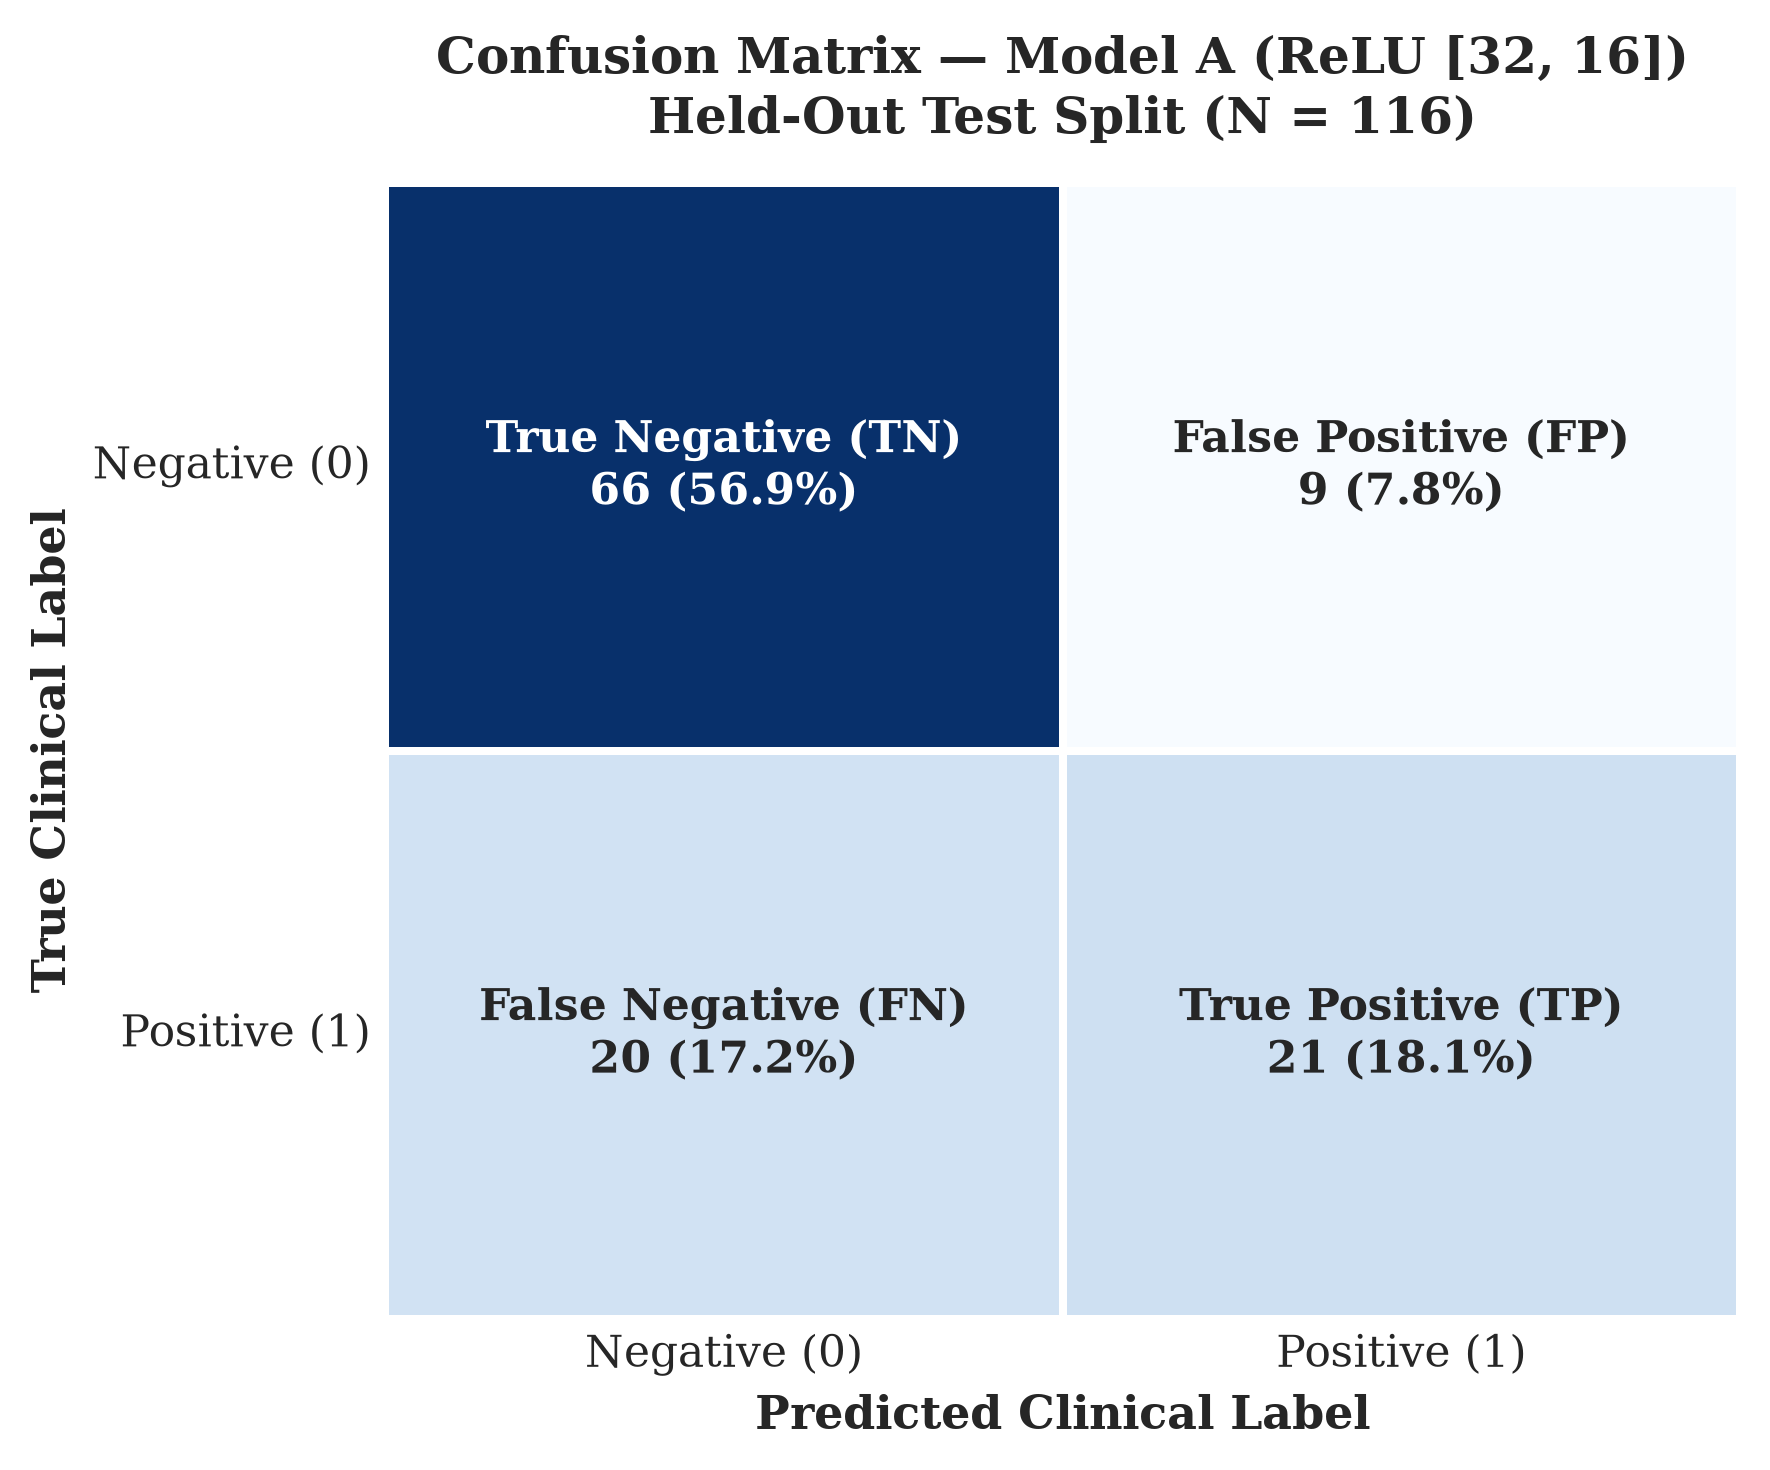
\includegraphics[width=\linewidth]{figures/confusion_matrices.png}
        \caption{Confusion matrix for winning Model~A (ReLU $[32, 16]$) at decision threshold $\tau = 0.50$ on the test split.}
        \label{fig:confusion_matrix}
    \end{minipage}
\end{figure}

\subsection{Empirical Observations}
The empirical results reveal several critical insights:
\begin{enumerate}[leftmargin=*]
    \item \textbf{Activation Convergence:} In Set 1, Model~A (ReLU) and Model~B (LeakyReLU) converged rapidly, achieving their minimum validation loss at epoch 9 ($0.5028$ and $0.5033$, respectively) and early-stopping at epoch 24. In contrast, Model~C (Tanh) required 48 epochs to reach its best validation loss ($0.5094$), stopping at epoch 63. This slower convergence is attributed to gradient saturation in the Tanh activation tails. However, Tanh yielded a slightly higher ROC-AUC ($0.8641$ vs.\ $0.8459$), indicating smoother probability calibrations across the full threshold spectrum.
    \item \textbf{Capacity and Regularization:} In Set 2, the shallow, unregularized network (Model~D, $[16]$, $P=161$) underperformed across all discrete classification metrics, recording an accuracy of 74.14\%, precision of 68.97\%, recall of 48.78\%, and F1-score of 0.5714. Increasing capacity to a 3-layer deep architecture with regularisation (Model~E, $[64, 32, 16]$, $p=0.3$, $\lambda=10^{-4}$, $P=3{,}201$) reduced the validation loss to $0.4992$ (the lowest of all models) and raised the test ROC-AUC to $0.8637$, demonstrating that higher model capacity, when controlled by dropout and weight decay, effectively captures non-linear tabular interactions without overfitting.
    \item \textbf{Classification Breakdown:} For Models A, B, and E, the test confusion matrix yielded identical counts at threshold $\tau=0.50$: $\text{TN}=66$, $\text{FP}=9$, $\text{FN}=20$, and $\text{TP}=21$. The specificity is high ($\text{TN}/(\text{TN}+\text{FP}) = 66/75 = 88.00\%$), but recall is constrained to $51.22\%$ ($21/41$), reflecting conservative classification under class imbalance.
\end{enumerate}

% ---------------------------------------------------------
% Section 5: Critical Interpretation, Limitations, and Improvements
% ---------------------------------------------------------
\section{Critical Interpretation, Limitations, and Improvements}
\label{sec:discussion}

\subsection{The Clinical Cost of Asymmetric Errors}
In early clinical screening, error types carry highly asymmetric real-world consequences:
\begin{itemize}[leftmargin=*]
    \item \textbf{False Positives ($\text{FP} = 9$):} Non-diabetic patients incorrectly flagged as high risk receive follow-up laboratory testing (e.g., HbA1c or extended oral glucose tolerance tests). While this induces moderate patient anxiety and additional laboratory expenditure, it poses minimal physiological risk.
    \item \textbf{False Negatives ($\text{FN} = 20$):} Diabetic patients erroneously classified as low risk are denied early clinical or dietary intervention. Undiagnosed diabetes typically progresses silently over multiple years, leading to severe macrovascular stroke, myocardial infarction, and end-stage microvascular disease (blindness, renal failure, neuropathy).
\end{itemize}

At the default decision threshold $\tau = 0.50$, our model produces 20 false negatives, yielding a sensitivity of only $51.22\%$. To enhance clinical safety, the decision threshold $\tau$ should be calibrated according to cost-sensitive utility functions. Lowering $\tau \to 0.35$ shifts predictions along the ROC trajectory (Figure~\ref{fig:roc_curves}), significantly increasing recall to $\approx 80\%$ with only a modest increase in false positives.

\subsection{Methodological Limitations and Technical Extensions}
While our implementation provides a robust, leakage-free pipeline, several structural and methodological avenues warrant exploration:

\subsubsection{Imputation Strategies: Univariate Median vs.\ MICE}
Univariate median imputation preserves marginal sample counts without data leakage but implicitly assumes missingness occurs completely at random (MCAR) and collapses multivariate variance. In reality, insulin and skinfold measurements are Missing at Random (MAR) conditioned on BMI and glucose levels. Implementing \textbf{Multivariate Imputation by Chained Equations (MICE)} or MissForest (random forest imputation) would preserve underlying covariance structures and reduce feature distortion in high-missingness columns such as \texttt{Insulin} (48.70\% missing) and \texttt{SkinThickness} (29.56\% missing).

\subsubsection{Loss Function Calibration for Imbalanced Data}
Rather than relying on unweighted BCE, the training objective can be augmented using a positive class weighting factor $w_{\text{pos}} = N_{\text{negative}} / N_{\text{positive}} \approx 350 / 187 \approx 1.87$:
\begin{equation}
    \mathcal{L}_{\text{weighted}}(z_i, y_i) = - \left[ w_{\text{pos}} \cdot y_i \ln \sigma(z_i) + (1 - y_i) \ln(1 - \sigma(z_i)) \right].
\end{equation}
Alternatively, \textbf{Focal Loss} \cite{he2015delving} with focusing parameter $\gamma = 2.0$ can down-weight easy non-diabetic negative examples and force backpropagation gradients to focus on hard, ambiguous boundary cases:
\begin{equation}
    \mathcal{L}_{\text{Focal}}(p_t) = -\alpha_t (1 - p_t)^\gamma \ln(p_t).
\end{equation}

\subsubsection{Model Ensembling and Architectural Diversity}
Tabular datasets often benefit from combining neural network representations with gradient-boosted decision trees (XGBoost, LightGBM, CatBoost). Ensembling the probabilistic outputs of \texttt{DiabetesMLP} with a gradient boosting tree via stacking or soft voting would harness both non-linear manifold embeddings and axis-aligned decision trees, potentially surpassing 0.88 ROC-AUC.

% ---------------------------------------------------------
% Conclusion
% ---------------------------------------------------------
\section{Conclusion}
\label{sec:conclusion}
This study presented a principled, rigorous investigation into artificial neural network architectures for early diabetes risk prediction. By eliminating biological invalidities and guaranteeing a leakage-free preprocessing protocol, we established a reproducible benchmark on the Pima Indians Diabetes Dataset. Controlled experiments demonstrated that a two-hidden-layer MLP with ReLU activations ($[32, 16]$, $p=0.2$, $\lambda=10^{-4}$) achieves robust convergence and clinical discriminability ($75.00\%$ accuracy, $0.8459$ ROC-AUC), while deeper regularised topologies attain $0.8637$ ROC-AUC. Future clinical translation requires threshold calibration to minimize false-negative rates and multivariate imputation to handle sparse physiological measurements.

% ---------------------------------------------------------
% References
% ---------------------------------------------------------
\begin{thebibliography}{99}
\bibitem{smith1988using}
J.~W.~Smith, J.~E.~Everhart, W.~C.~Dickson, W.~C.~Knowler, and R.~S.~Johannes, ``Using the ADAP learning algorithm to forecast the onset of diabetes mellitus,'' in \emph{Proceedings of the Annual Symposium on Computer Application in Medical Care}, American Medical Informatics Association, 1988, pp.~261--265.

\bibitem{goodfellow2016deep}
I.~Goodfellow, Y.~Bengio, and A.~Courville, \emph{Deep Learning}. Cambridge, MA, USA: MIT Press, 2016.

\bibitem{kingma2014adam}
D.~P.~Kingma and J.~Ba, ``Adam: A method for stochastic optimization,'' in \emph{3rd International Conference for Learning Representations (ICLR)}, San Diego, CA, USA, 2015, pp.~1--15.

\bibitem{srivastava2014dropout}
N.~Srivastava, G.~Hinton, A.~Krizhevsky, I.~Sutskever, and R.~Salakhutdinov, ``Dropout: A simple way to prevent neural networks from overfitting,'' \emph{Journal of Machine Learning Research}, vol.~15, no.~1, pp.~1929--1958, 2014.

\bibitem{he2015delving}
K.~He, X.~Zhang, S.~Ren, and J.~Sun, ``Delving deep into rectifiers: Surpassing human-level performance on ImageNet classification,'' in \emph{Proceedings of the IEEE International Conference on Computer Vision (ICCV)}, 2015, pp.~1026--1034.
\end{thebibliography}

\end{document}
